\documentclass[11pt]{scrartcl}

\usepackage{ucs}
\usepackage[utf8x]{inputenc}
\usepackage{ngerman}
\usepackage{amsmath,amssymb,amstext}
\usepackage{graphicx}
\usepackage[automark]{scrpage2}
\usepackage{pgfplots}
\usepackage{chngcntr}
\usepackage[left=3cm, right=3cm, top=3cm, bottom=3cm]{geometry}
\counterwithin{figure}{section}

\pagestyle{scrheadings}

\title{Radixsort}
\author{Finn Jannsen, Philipp Schwarz}
\date{\today{}}

\begin{document}

\maketitle

\tableofcontents

\section{Einführung}
	\label{sec:einfuehrung}
	
	Diese Dokumentation beschreibt eine Sortieralgorithmus-Implementation für Arrays mit vordefinierten Integer-Keys, basierend auf Radixsort.
	In Abschnitt \ref{sec:implementation} wird darauf eingegangen, wie der Algorithmus realisiert wurde.
	Anschließend wird in Abschnitt \ref{sec:veri} geprüft, ob die Implementation korrekt funktioniert 
	und in Abschnitt \ref{sec:aufwand} die Performance mit dem zu Grunde liegenden Quicksort verglichen.

\section{Implementation}
	\label{sec:implementation}
	
	Der Algorithmus wurde als Klasse realisiert, der ein Interface implementiert, welches es ermöglicht, einfach weitere Implementationen, sofern dies gewünscht wird, zu schreiben.
	
	\subsection{Sortieren}
		\label{sec:sortAlgo}
		
		Der bisherige Quicksort-Algorithmus besteht im wesentlichen aus einer Schleife, in der zuerst das erste Element von links, welches gleich oder größer als Pivot ist, gesucht wird.
		Danach wird das erste Element von rechts, welches kleiner als das Pivot ist, gesucht. Diese werden dann getauscht.
		Die Schleife wird verlassen, wenn die jeweiligen Such-Schleifen einander kreuzen.
		Danach wird das Pivot in diese Mitte an Stelle i zurückgetauscht und der Algorithmus wird zwei mal rekursiv gestartet,
		einmal um die Liste von ganz links bis i-1 zu sortieren und noch einmal um die Liste von i+1 bis rechts zu sortieren.

		Radixsort besteht aus mehreren Schritten, und jeder Schritt aus zwei Phasen. 
        Die Partitionierungsphase dient dazu, die Daten auf Fächer aufzuteilen, während in der Sammelphase die Daten aus diesen Fächern wieder aufgesammelt werden. 
        Beide Phasen werden für jede Stelle des zu sortierenden Schlüssels einmal durchgeführt. Die Anzahl der Schritte ist gleich der maximalen Stellenanzahl. 

		Der Code hierfür ist in \ref{figure:sortCode} dargestellt.

\section{Testen und Verifikation}
\label{sec:vertests}

	\subsection{Verifizieren}
		\label{sec:veri}
		
		Der Algorithmus wurde auf seine korrekte Funktionalität getestet.
		Hierzu zählt natürlich das Vorliegen des Ergebnisses in der korrekten Reihenfolge.
		Alle Tests wurden erfolgreich mit unterschiedlichen Eingabewerten absolviert.
	
	\subsection{Aufwandsanalyse}
		\label{sec:aufwand}
		
		Für die Aufwandsanalyse wurde der Klasse ein Counter eingeführt, der die Tauschoperationen zählt, als auch die Ausführungszeit beobachtet. 
		
		Bisherige Untersuchungen von Quicksort haben bereits einen Asymptotischen Aufwand wie folgt ergeben:

		Rechenoperationen bei Best- und Average Case:
		\begin{equation*}
		T(n) = \mathcal{O}(n*ln(n))
		\end{equation*}
		Rechenoperationen bei Worst Case:
		\begin{equation*}
		T(n) = \mathcal{O}(n^{2})
		\end{equation*}

		Bei der Radixsort-Implementation ist der Asymptotische Aufwand konstant wie folgt (l ist die Länge des Keys):
		\begin{equation*}
		T(n) = \mathcal{O}(l*n)
		\end{equation*}
        
		Außerdem wurden dieses mal statt komplett zufälligen Key-Werten welche mit folgender Beschränkung ausgewählt: 
		\begin{equation*}
		700*N \leq key \leq 800*N
		\end{equation*}
        
		Es wurden 10 Durchläufe des Tests mit den Größen $N=10^k, k=1,...,6$ durchgeführt, um einen angemessenen Mittelwert zu ermitteln.

		Die Ergebnisse für die Rechenoperationen sind in Abbildung \ref{figure:ranOperTest} zu sehen.
		Es ist ersichtlich, dass das Radixsort weniger Rechenoperationen verursacht.

\begin{figure}
    \newcommand{\rsCol}{blue}
    \newcommand{\qsCol}{red}
    \newcommand{\bestAvgMark}{square*}
    \newcommand{\transparent}{0.8}
    \makebox[\textwidth][c]{
    \begin{tikzpicture}
        \begin{loglogaxis}[
                title={\large Berechnung Operationen},
                height=10cm,
                width=17cm,
                grid=major,
                x tick label style={
                /pgf/number format/1000 sep=},
                ylabel=Operationen,
                xlabel=Anzahl Elemente,
                enlargelimits=0.05,
                legend style={at={(0.5,-0.15)},
                anchor=north,legend columns=1},
            ]
            \addplot[color=\rsCol,mark=\bestAvgMark,opacity=\transparent]
                coordinates {(1,0)(10,116)(100,1045)(1000,12054)(10000,140063)(100000,1600072)(1000000,18000081)};
            \addplot[color=\qsCol,mark=\bestAvgMark,opacity=\transparent]
                coordinates {(1,0)(10,21.05)(100,562.34)(1000,9445.31)(10000,133652.47)(100000,1731953.94)(1000000,21272971.31)};
            \legend{Radixsort, Quicksort}
        \end{loglogaxis}
    \end{tikzpicture}
    }
    \caption{Quantitativer Vergleich zu Quicksort anhand Rechenoperationen}
    \label{figure:ranOperTest}
\end{figure}

\begin{figure}
\begin{verbatim}
Node[] out = new Node[list.length];

int[] count = new int[10];

for (int i = 0; i < list.length; i++) {
    int digit = getDigit(list[i].getKey(), exp);
    count[digit] += 1;
}

for (int i = 1; i < count.length; i++) {
    count[i] += count[i - 1];
}

for (int i = list.length - 1; i >= 0; i--) {
    int digit = getDigit(list[i].getKey(), exp);

    out[count[digit] - 1] = list[i];
    count[digit]--;
}

return out;
\end{verbatim}
\caption{Code-Ausschnitt Sortieren}
\label{figure:sortCode}
\end{figure}

\begin{figure}
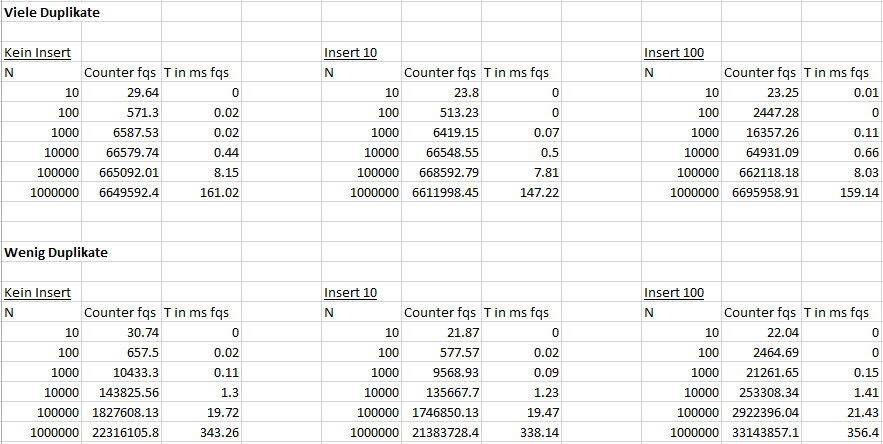
\includegraphics[width=\linewidth]{insertiontable.png}
\caption{Durchschnittswerte unterschiedlicher Insertionsorts von 100 Durchführungen bei vielen und wenigen Duplikaten}
\label{figure:table}
\end{figure}
\end{document}